% ============================================================
% TEMPLATE: Standalone TikZ Figure
% Dùng cho: Vẽ một hình đơn lẻ, export ra PDF/PNG
% ============================================================

\documentclass[tikz,border=5pt]{standalone}

% === ENCODING ===
\usepackage[utf8]{inputenc}
\usepackage[T5]{fontenc}  % Vietnamese support

% === TIKZ & LIBRARIES ===
\usepackage{tikz}
\usetikzlibrary{
    calc,                   % Tính toán tọa độ
    arrows.meta,            % Mũi tên đẹp
    angles,                 % Đánh dấu góc
    quotes,                 % Nhãn góc
    positioning,            % Vị trí tương đối
    patterns,               % Mẫu tô (gạch chéo)
    shapes.geometric,       % Hình học
    decorations.pathmorphing, % Sóng, lò xo
    decorations.markings,   % Đánh dấu trên đường
}

% === PGFPLOTS (cho đồ thị) ===
\usepackage{pgfplots}
\pgfplotsset{compat=1.18}

% === CHEMFIG (cho Hóa học) ===
\usepackage{chemfig}

% === CIRCUITIKZ (cho mạch điện) ===
\usepackage{circuitikz}

% ============================================================
% ĐỊNH NGHĨA STYLE CHUNG
% ============================================================
\tikzset{
    % Style cho điểm
    point/.style={circle, fill, inner sep=1.5pt},
    % Style cho đường chính
    main line/.style={thick},
    % Style cho đường phụ
    aux line/.style={thin, dashed, gray},
    % Style cho vector
    vector/.style={-{Stealth[length=3mm]}, thick},
}

% ============================================================
\begin{document}
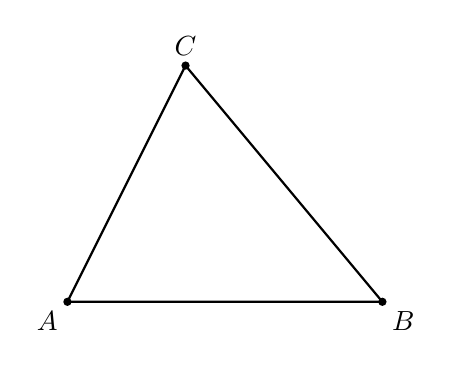
\begin{tikzpicture}[
    % Có thể thêm options ở đây
    % scale=1.2,
]

% === CODE VẼ HÌNH Ở ĐÂY ===

% Ví dụ: Tam giác ABC
\coordinate (A) at (0,0);
\coordinate (B) at (4,0);
\coordinate (C) at (1.5,3);

% Vẽ tam giác
\draw[main line] (A) -- (B) -- (C) -- cycle;

% Nhãn
\node[below left] at (A) {$A$};
\node[below right] at (B) {$B$};
\node[above] at (C) {$C$};

% Đánh dấu điểm
\foreach \p in {A,B,C} \fill (\p) circle (1.5pt);

% === KẾT THÚC CODE ===

\end{tikzpicture}
\end{document}
